\chapter*{Management Summary}

\section*{Scoreboard}
In a game of Coiffeur Jass there are many things to keep track of:

\begin{itemize}
    \item Round scores
    \item Multipliers
    \item Total Scores
    \item Who gets to choose the next contract
\end{itemize}

All of this is difficult to keep track of in your head. That's why traditionally a chalkboard is used to keep track of what has been played. JassTracker is a web-based replacement for the classic chalkboard and more. With JassTracker you only need to enter the score of each round and our dynamic scoreboard will take care of the rest. The scoreboard also highlights who picks the contract for the next round, so you never have to count the rounds in your head again.

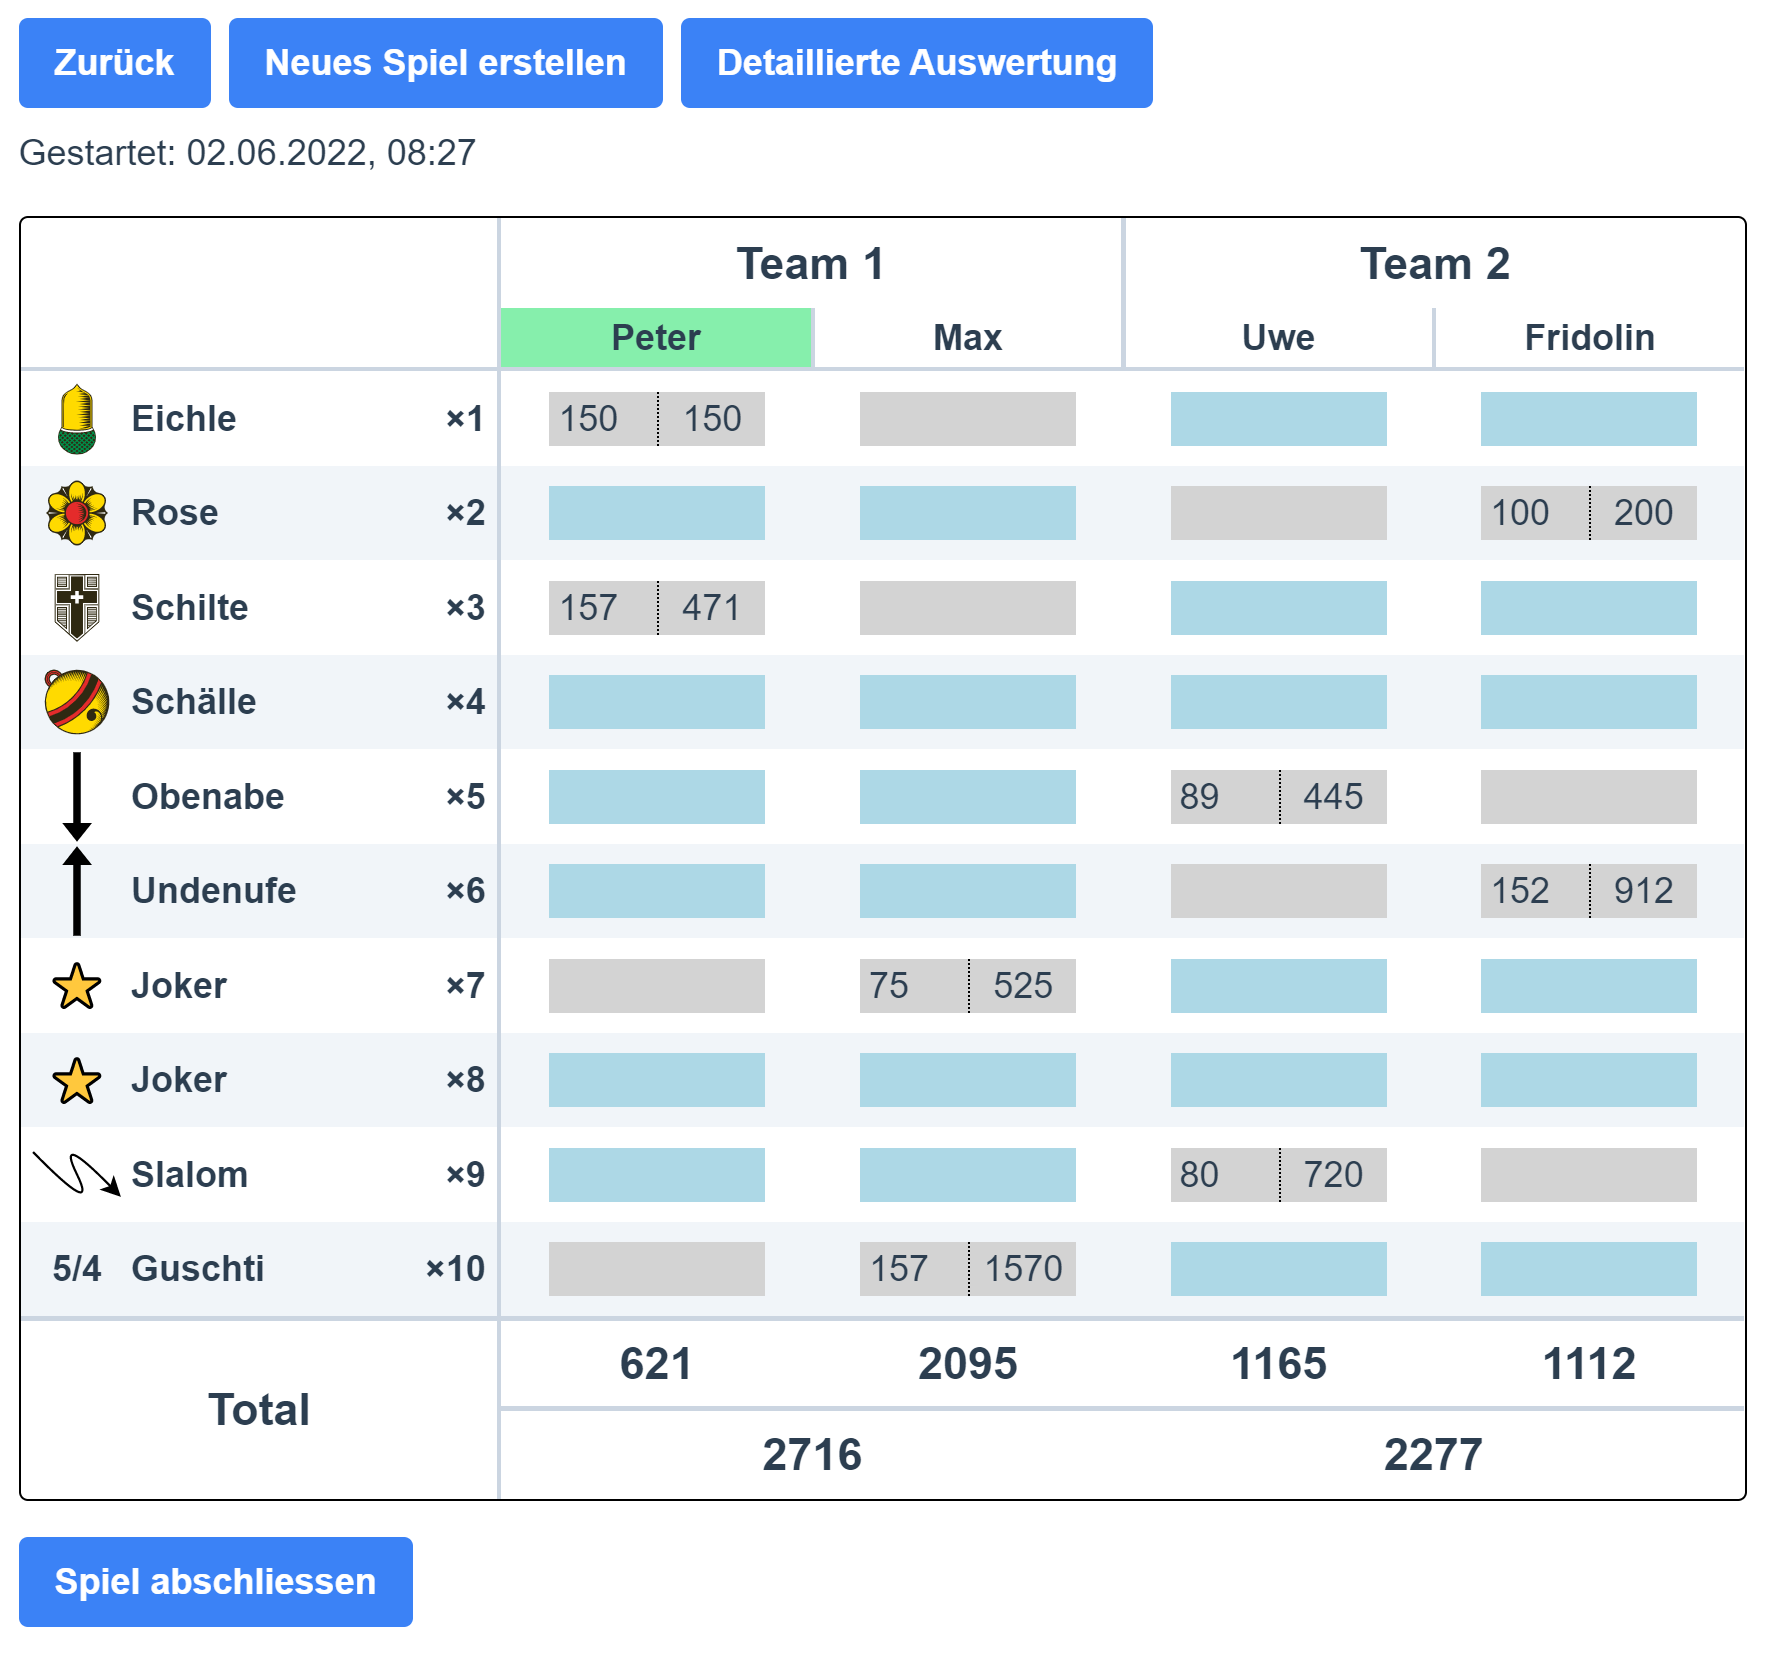
\includegraphics[height=0.4\textheight]{resources/screenshots/scoreboard}

\section*{Tables}
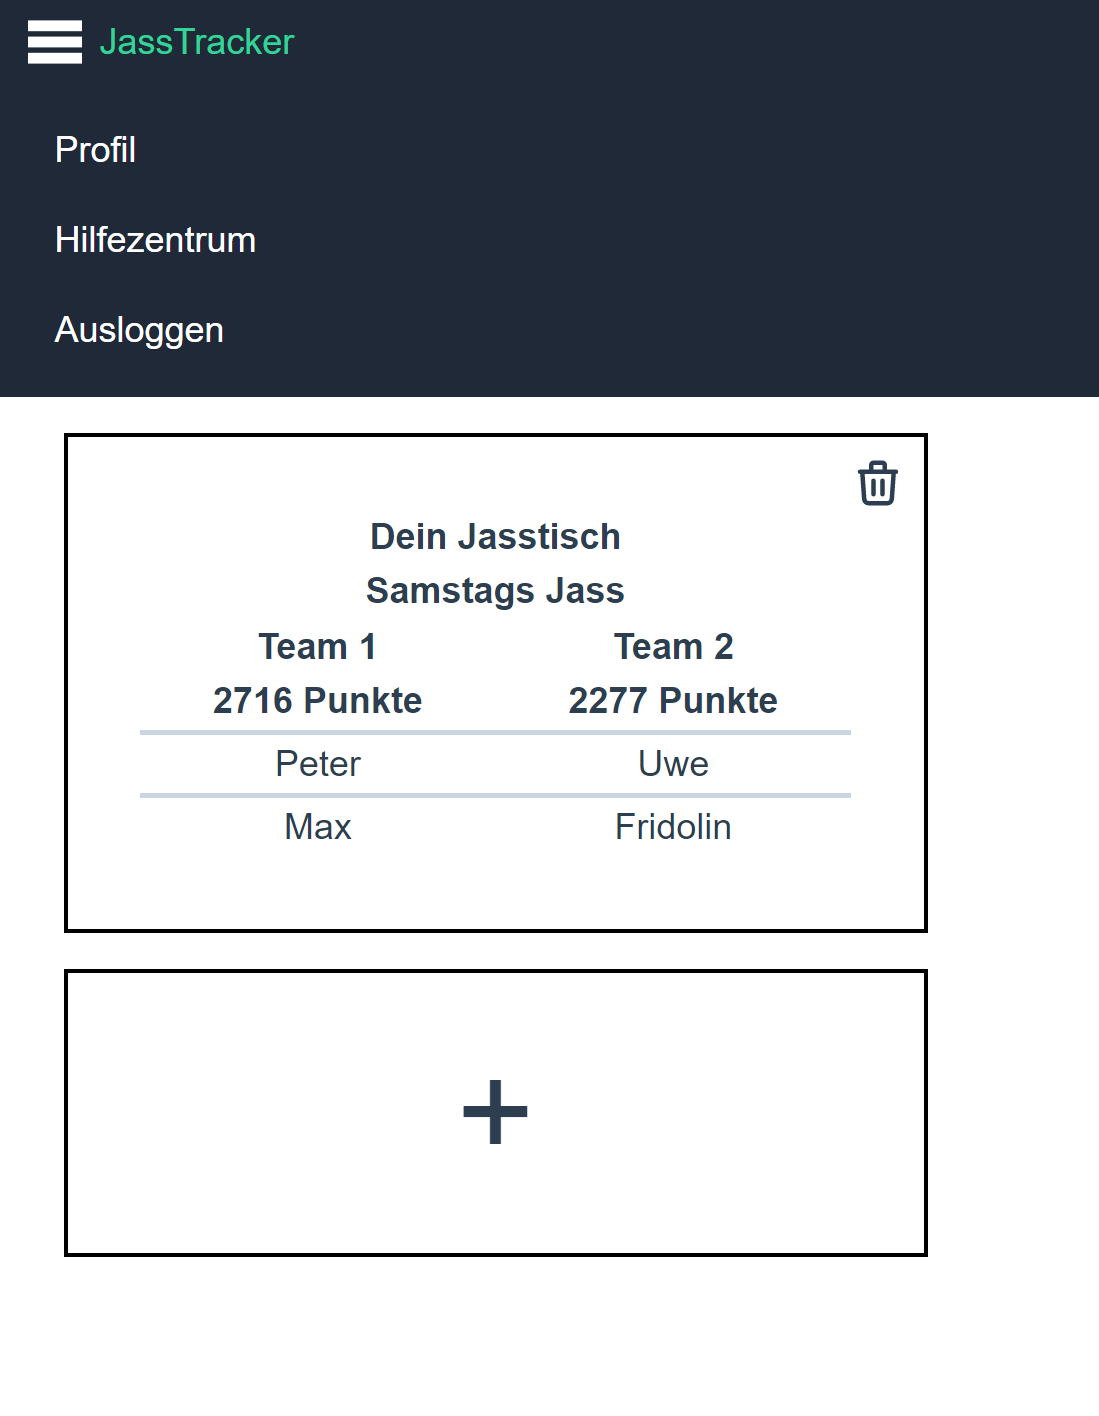
\includegraphics[height=0.5\textheight]{resources/screenshots/tables}

If you are playing Jass with several groups of people, e.g. your family or a group of friends, it would be nice if you could separate the games. For this we introduce the concept of a Jass table, which allows you to group your Jass games. The table creation dialog allows you to add players to the table and to play around with different team constellations.

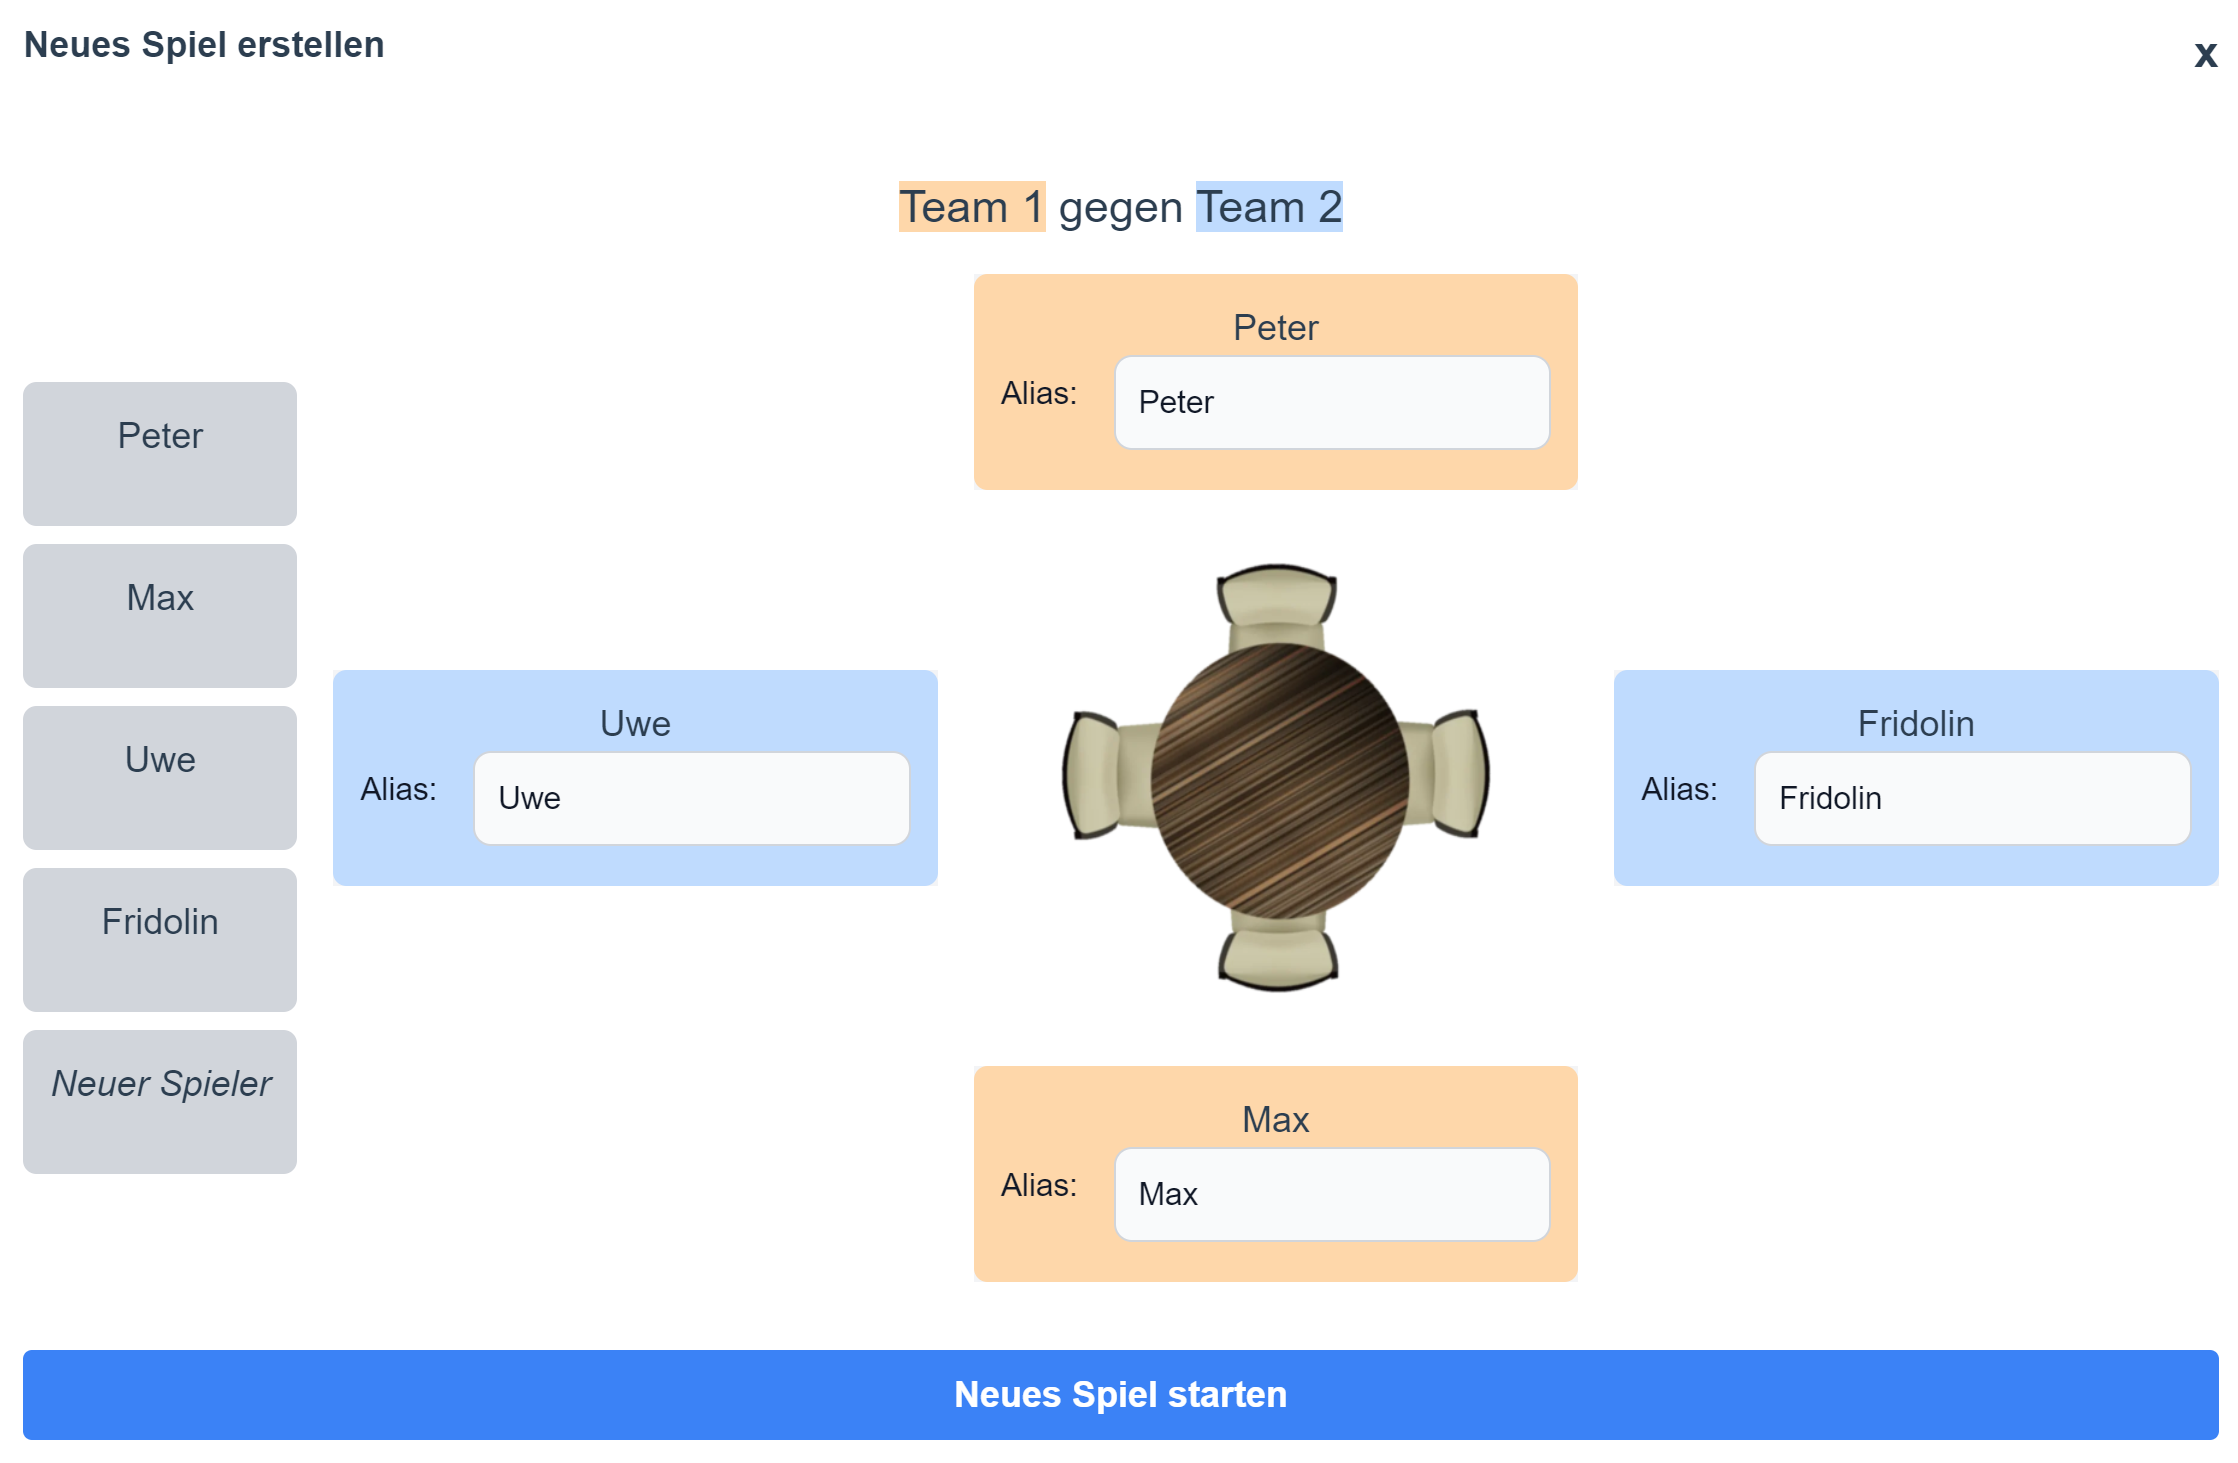
\includegraphics[width=0.9\textwidth]{resources/screenshots/table-creation}

\section*{Statistics}
JassTracker offers statistics at different levels of granularity. You can view the statistics for a single game, but perhaps more interesting are the statistics at the table level. After dozens of matches with your family, you can finally settle who is the best Jasser in the family, thanks to JassTracker.

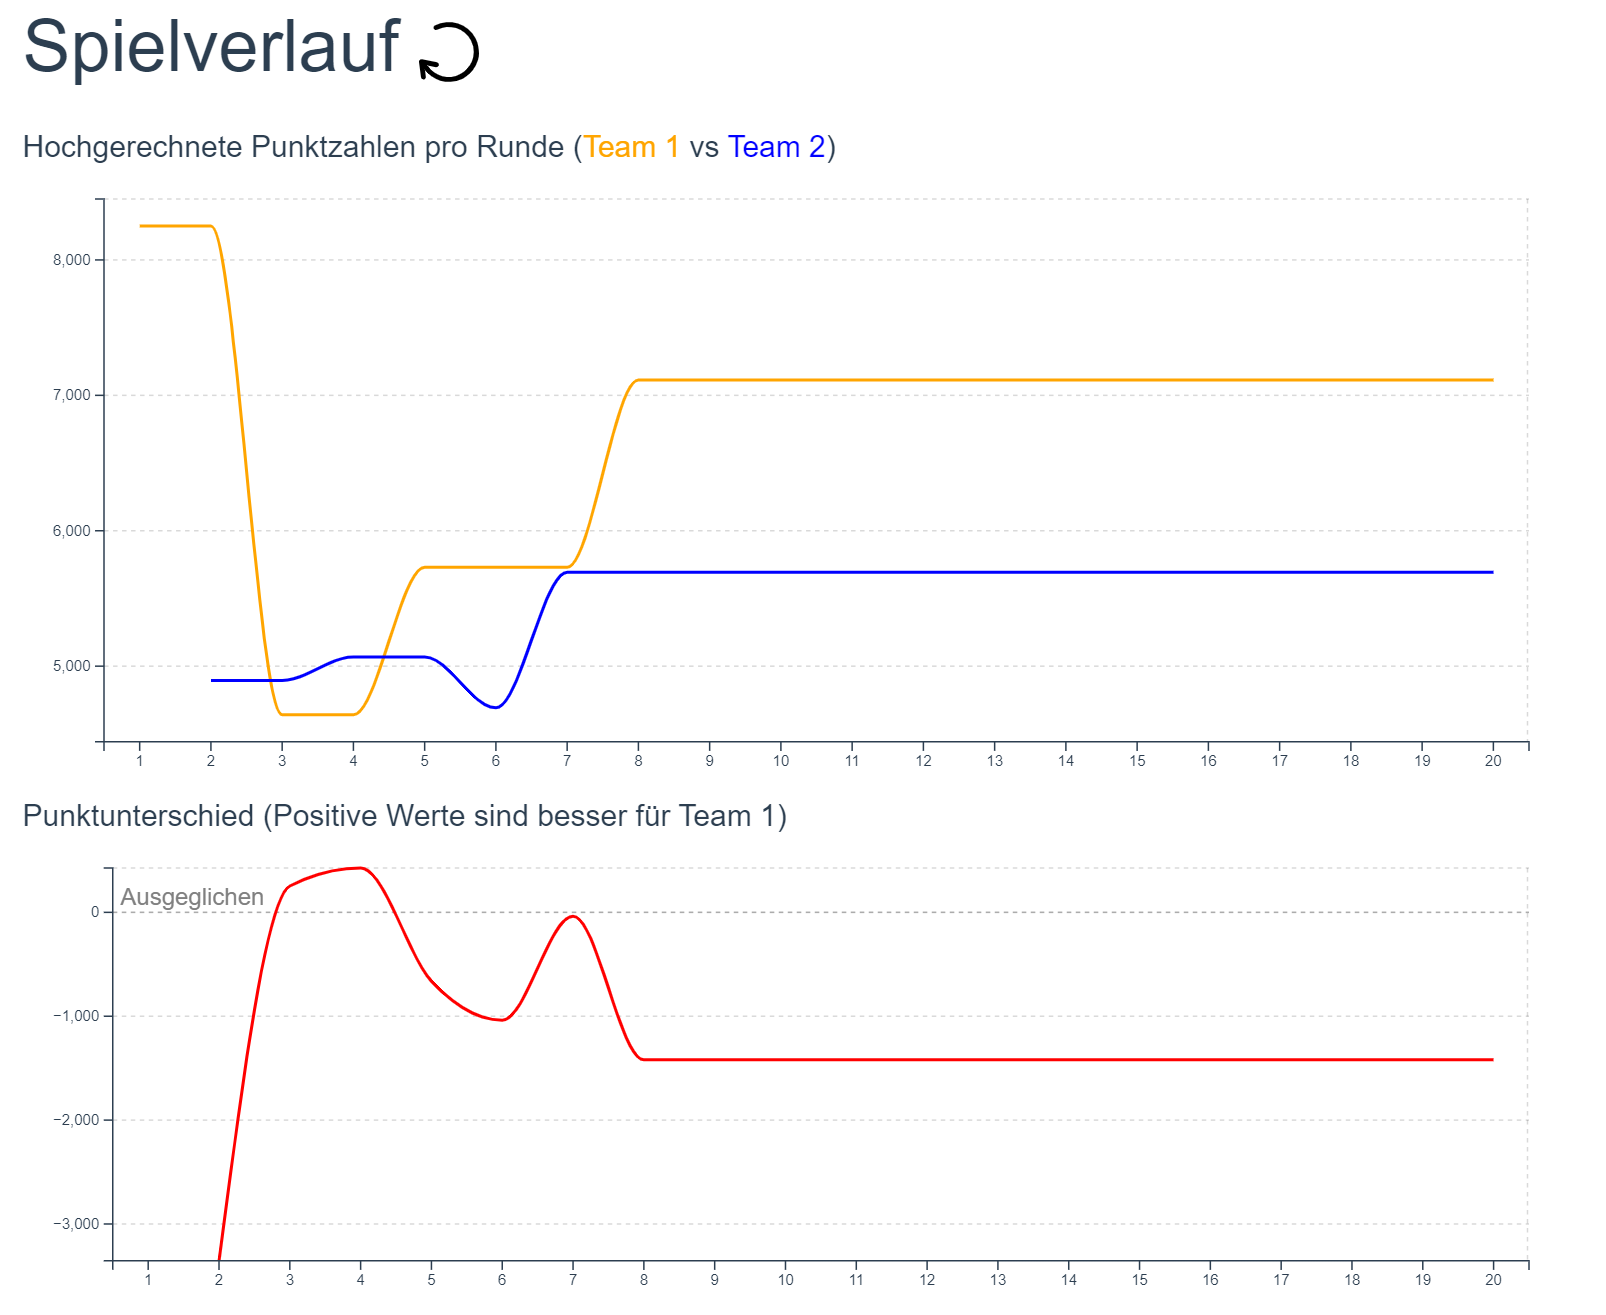
\includegraphics[width=0.9\textwidth]{resources/screenshots/statistics}

\section*{Profile}
If you register with JassTracker instead of playing as a guest, you will never lose access to your games. On top of that you get access to your individual statistics, which will show you just how good you are at Jass. You can also set your display name, which is entered by default when you create a new game. However it can be changed for each game. So if you find yourself playing Jass with shady figures who should not know your true identity, we've got your back.
